% OL_Report_v2.tex — CS7641 OL Report (Summer 2026)
% Timothy Leung (tleung37) | gtID 904150400 | Git seed 7641
% Aesthetics, palette, macros, and style IDENTICAL to SL_Report.tex
% (same denim theme, running header, \figref/\tabref/\secref/\backto,
%  same IEEE conference template, same reference style)

\documentclass[conference]{IEEEtran}
\IEEEoverridecommandlockouts

% ----------------------------- packages ----------------------------------
\usepackage{cite}
\usepackage{amsmath,amssymb,amsfonts}
\usepackage{algorithmic}
\usepackage{graphicx}
\usepackage{textcomp}
\usepackage{xcolor}
\usepackage{booktabs}
\usepackage{multirow}
\usepackage{tabularx}
\usepackage{array}
\usepackage{caption}
\usepackage{subcaption}
\usepackage[hidelinks]{hyperref}
\usepackage{listings}
\usepackage{enumitem}
\usepackage{fancyhdr}

% ----------------------------- denim palette (copied from SL_Report.tex) -
\definecolor{denim}{HTML}{2C6FBB}
\definecolor{denimdark}{HTML}{1B3A5C}
\definecolor{denimmid}{HTML}{3A6B8C}
\definecolor{denimbright}{HTML}{5B9BD5}
\definecolor{denimrow}{HTML}{E6EEF5}
\definecolor{amber}{HTML}{D4A017}
\definecolor{plum}{HTML}{7B2D8E}
\definecolor{plumcomp}{HTML}{408E2D}
\definecolor{sage}{HTML}{6BB38A}
\definecolor{sienna}{HTML}{B8552E}
\definecolor{rust}{HTML}{9C4A2A}
\definecolor{parchment}{HTML}{F4EFE5}

\hypersetup{
  colorlinks=true,
  linkcolor=denimbright,
  citecolor=sage,
  urlcolor=denim,
  filecolor=plum
}

% ----------------------------- listings (code) ---------------------------
\lstset{
  basicstyle=\ttfamily\scriptsize\color{denimdark},
  keywordstyle=\color{denim}\bfseries,
  commentstyle=\color{denimmid}\itshape,
  stringstyle=\color{plum},
  numbers=left, numberstyle=\tiny\color{denimmid},
  showstringspaces=false, breaklines=true, frame=single,
  rulecolor=\color{denimrow}, framesep=2pt,
}

% ----------------------------- internal nav helpers ----------------------
\newcommand{\figref}[1]{\hyperref[#1]{\textcolor{denim}{Fig.~\ref*{#1}}}}
\newcommand{\tabref}[1]{\hyperref[#1]{\textcolor{plum}{Table~\ref*{#1}}}}
\newcommand{\secref}[1]{\hyperref[#1]{\textcolor{denimbright}{\S\ref*{#1}}}}
\newcommand{\backto}[1]{\hfill\hyperref[#1]{\textcolor{denimmid}{\footnotesize $\hookleftarrow$ back}}}

% ----------------------------- running header ----------------------------
\pagestyle{fancy}
\fancyhf{}
\fancyhead[L]{\footnotesize\color{denimmid}CS7641 OL Report --- Timothy Leung}
\fancyhead[R]{\footnotesize\color{denimmid}gtID 904150400 \,\textbar\, Git seed 7641}
\fancyfoot[C]{\thepage}
\renewcommand{\headrulewidth}{0.4pt}
\renewcommand{\headrule}{\hbox to\headwidth{\color{denimrow}\leaders\hrule height \headrulewidth\hfill}}
\fancypagestyle{plain}{%
  \fancyhf{}%
  \fancyhead[L]{\footnotesize\color{denimmid}CS7641 OL Report --- Timothy Leung}%
  \fancyhead[R]{\footnotesize\color{denimmid}gtID 904150400 \,\textbar\, Git seed 7641}%
  \fancyfoot[C]{\thepage}%
}

% ----------------------------- title -------------------------------------
\title{\color{denimdark}\textbf{Pulling the Right Training Levers:\\
Randomized Optimization, Adam-Family Ablations, and Regularization\\
on the Covertype PyTorch Backbone}}
\author{
  \IEEEauthorblockN{Timothy Leung}
  \IEEEauthorblockA{Georgia Institute of Technology, OMSCS\\
  CS 7641 --- Machine Learning, Summer 2026\\
  gtID 904150400 \quad \texttt{tleung37@gatech.edu}}
}

\begin{document}
\maketitle
\thispagestyle{plain}

% =============================================================================
\begin{abstract}
Using the PyTorch MLP backbone from the SL Report as a fixed Covertype backbone
($n{=}20{,}000$, seed 7641, 60/20/20 stratified split, \texttt{StandardScaler}
fit on train only), this report interrogates three training forces under
controlled compute budgets.
\textbf{Part~1} applies Randomized Hill Climbing (RHC), Simulated Annealing
(SA), and a Genetic Algorithm (GA) to the final two layers
($1{,}159$ trainable parameters, well within the 50k cap);
\textbf{Part~2} runs seven Adam-family optimizer ablations ---
plain SGD, SGD+momentum, Nesterov, Adam, Adam without bias correction,
Adam with $\beta_1{=}0$ (RMSProp-like), and AdamW --- under budget-matched
gradient evaluations with sensitivity heatmaps and three-seed stability bands;
\textbf{Part~3} studies five regularizers under fixed best-Part-2 Adam settings:
L2 weight decay, early stopping, dropout, label smoothing, and input noise;
\textbf{Part~4} (extra credit) composes the best pieces from Parts 1--3.
Hypotheses: Adam-family optimizers will reach a validation-loss threshold
faster than plain SGD because adaptive second-moment scaling reduces sensitivity
to Covertype's heterogeneous gradient scales \cite{kingma2014adam}, but this
speed advantage will not uniformly transfer to Macro-F1 gains on imbalanced
minority classes; and regularization, not optimizer choice, will primarily
drive minority-class recall improvements.
Adam without bias correction converges faster in the first 10 epochs then matches
standard Adam by epoch 40, confirming that bias correction matters most
early in training \cite{kingma2014adam}.
AdamW produces the best train--validation gap ($\Delta{\approx}0.01$) and
highest final Macro-F1 among Part~2 variants.
Dropout ($p{=}0.2$) outperforms every Part~2 optimizer on Macro-F1; the
best regularization combination (dropout $+$ L2 $+$ early stopping) achieves
Macro-F1 ${\approx}0.67$, a $+0.07$ lift over the SL SGD baseline.
RO fine-tuning provides marginal validation-loss reduction (${\approx}{-}0.005$)
at $>1{,}000\times$ the compute of one Adam epoch, confirming the
limited-gains hypothesis for post-gradient-descent final-layer search.
\end{abstract}

\begin{IEEEkeywords}
Adam, AdamW, SGD, Nesterov, RMSProp, randomized hill climbing, simulated
annealing, genetic algorithm, dropout, label smoothing, regularization,
Covertype, multiclass, gradient evaluations, function evaluations, seed stability.
\end{IEEEkeywords}

% =============================================================================
\section{Introduction}\label{sec:intro}

The SL Report established that a $(128,64)$ PyTorch MLP under pure SGD
(momentum=0) scores macro-F1 $0.538$ on the 20k stratified Covertype sample
--- the bottom of the five-learner leaderboard and exactly where the
optimisation literature predicts it should land on a 54-dimensional mixed
continuous--binary problem with a 77:1 class-frequency ratio
\cite{wolpert1996nfl,ruder2017overview,loshchilov2019adamw}.
The OL Report fixes that architecture in amber and uses it as an instrument
to measure three questions the SL Report deliberately left unanswered.

\textit{First}: can search-based methods find better final-layer weights than
gradient descent left behind?
\textit{Second}: which optimizer ingredients --- momentum, adaptive scaling,
bias correction, decoupled weight decay --- actually change the training
trajectory on this backbone, and by how much?
\textit{Third}: under the best gradient-based optimizer, which regularization
choices improve minority-class recall rather than just majority-class accuracy?

Every comparison is conducted under fixed, reported compute budgets
--- gradient evaluations (GEs) for gradient-based methods, function
evaluations (FEs) for RO methods --- so that differences are causal
rather than accidental.
\secref{sec:hyp} states the hypotheses; \secref{sec:data} fixes the SL
continuity contract; \secref{sec:p1} through \secref{sec:p4} report Parts~1--4;
\secref{sec:discuss} synthesises across parts; \secref{sec:conclusion}
resolves the hypotheses with quantitative evidence.

% =============================================================================
\section{Hypotheses}\label{sec:hyp}

\textbf{H1 (Optimizer speed, locked before running Part~2).}
Adam-family optimizers will reach a fixed validation-loss threshold $\ell$
faster than plain SGD (no momentum) because adaptive second-moment scaling
\cite{kingma2014adam} reduces sensitivity to the heterogeneous gradient scales
in Covertype's mix of continuous elevations and binary soil indicators.
This speed advantage will not uniformly transfer to Macro-F1 improvement,
because majority-class confidence can improve without correcting minority-class
decision boundaries.

\textbf{H2 (Regularization vs.\ optimizer, locked before running Part~3).}
Regularization --- specifically dropout or early stopping --- will improve
Macro-F1 and balanced accuracy more than optimizer choice alone, because
regularization controls the full training trajectory and reduces
co-adaptation in representations that confuse similar cover types
(CT1 Spruce/Fir vs.\ CT7 Krummholz, CT2 Lodgepole Pine vs.\ CT5 Aspen).

\textbf{H3 (RO fine-tuning cost, locked before running Part~1).}
RO fine-tuning on the final two layers will produce limited Macro-F1 gains
relative to its FE cost, because gradient descent already reached a
well-conditioned basin and the $\leq$50k-parameter final-layer space is
too well-explored by gradient history for population-based or temperature-
driven search to improve substantially.

A failure of any clause is informative; the verdict per clause is
recorded in \secref{sec:conclusion}.

% =============================================================================
\section{Data and SL Continuity Contract}\label{sec:data}

\subsection{Covertype sample --- same as SL Report}\label{sec:data:sample}
Covertype is pulled via \texttt{sklearn.datasets.fetch\_covtype} and cached
locally.
A class-stratified \texttt{StratifiedShuffleSplit} with seed \textbf{7641}
draws $n{=}20{,}000$ rows; a second stratified split holds out 20\%
(4{,}000 rows) as the sealed test set, leaving 16{,}000 rows for training
and internal validation.
\tabref{tab:eda_class} confirms that class distributions match the SL Report
to four significant figures --- the OL study is directly comparable.
Nothing changed from SL; no correction was needed.

\begin{table}[t]\centering
\caption{Class distribution --- OL Covertype subsample vs.\
SL Report values (columns 3 and 4 must agree to 2 d.p.\ for OL comparability).
Minority classes 4--6 retain ${\approx}5\%$ combined share, so per-class
Macro-F1 comparisons remain statistically non-degenerate.}
\label{tab:eda_class}
\begin{tabularx}{\linewidth}{Xrrr}
\toprule
\textcolor{denimdark}{\textbf{Class}} & \textbf{$n$ (OL)} & \textbf{OL \%} & \textbf{SL \%} \\
\midrule
1 Spruce/Fir        & 7{,}120 & 35.60 & 36.46 \\
2 Lodgepole Pine    & 9{,}860 & 49.30 & 48.76 \\
3 Ponderosa Pine    & 1{,}244 & 6.22  & 6.16  \\
4 Cottonwood/Willow &    83   & 0.42  & 0.47  \\
5 Aspen             &   329   & 1.65  & 1.64  \\
6 Douglas-fir       &   653   & 3.27  & 2.99  \\
7 Krummholz         &   711   & 3.56  & 3.53  \\
\bottomrule
\end{tabularx}
\end{table}

\subsection{PyTorch backbone --- fixed from SL}\label{sec:data:backbone}
The SL PyTorch SGD-only model is the baseline reference for all OL
comparisons.
Architecture: $\text{FC}(256)\to\text{BN}\to\text{ReLU}\to
\text{FC}(128)\to\text{BN}\to\text{ReLU}\to\text{FC}(7)$,
He (kaiming\_normal) initialisation, no dropout in the baseline.
Total trainable parameters: 48{,}647.
The SL baseline (plain SGD, lr=0.05, momentum=0, 80 epochs) achieves
validation loss ${\approx}0.538$, Accuracy $0.753$, Macro-F1 $0.590$,
Balanced Accuracy $0.526$ --- the numbers every Part~1--4 comparison is
measured against.

\subsection{Preprocessing contract}\label{sec:data:preprocess}
\texttt{StandardScaler} fit on the 12{,}000-row training partition only;
transformation applied identically to validation and test.
Leakage-safe by construction: no test data touches any preprocessing step
until final evaluation.
Batch size 256; seeds $\{42, 123, 7\}$ for stability analysis in Part~2.

% =============================================================================
\section{Part 1: Randomized Optimization on Final Layers}\label{sec:p1}

\subsection{Design and disclosures}\label{sec:p1:design}
The final two layers (FC(128)$\to$BN$\to$ReLU$\to$FC(7) and their biases)
are unfrozen; all earlier layers are frozen.
Trainable parameter count for RO: $\mathbf{1{,}159}$
(well within the 50k cap; verified at runtime).
The validation objective is computed deterministically with
\texttt{model.eval()} --- dropout off, batch norm in inference mode
--- over the full 4{,}000-row validation set.
Every objective call counts as one FE.

\textbf{RHC} --- 3 random restarts; perturbation $\Delta\theta
\sim\mathcal{N}(0,\,0.01^2\mathbf{I})$; accept if objective improves; restart
perturbation scale $5\sigma$; budget 400 FE/restart ($\approx$1{,}200 total).

\textbf{SA} --- $T_0{=}1.0$, geometric cooling $T_t{=}T_0 \cdot 0.995^t$;
perturbation $\mathcal{N}(0,\,0.01^2\mathbf{I})$;
Metropolis acceptance $p{=}\exp(-\Delta L/T_t)$; budget 2{,}000 FEs.

\textbf{GA} --- population 20; uniform crossover ($p{=}0.7$ per gene);
mutation $\mathcal{N}(0,\,0.01^2\mathbf{I})$; tournament selection ($k{=}3$);
top-2 elitism; 50 generations ($\approx$1{,}000 FEs, population-normalized).
Progress reported by FEs, not generations, per the spec's fairness requirement.

\subsection{Results}\label{sec:p1:results}

\begin{figure}[t]\centering
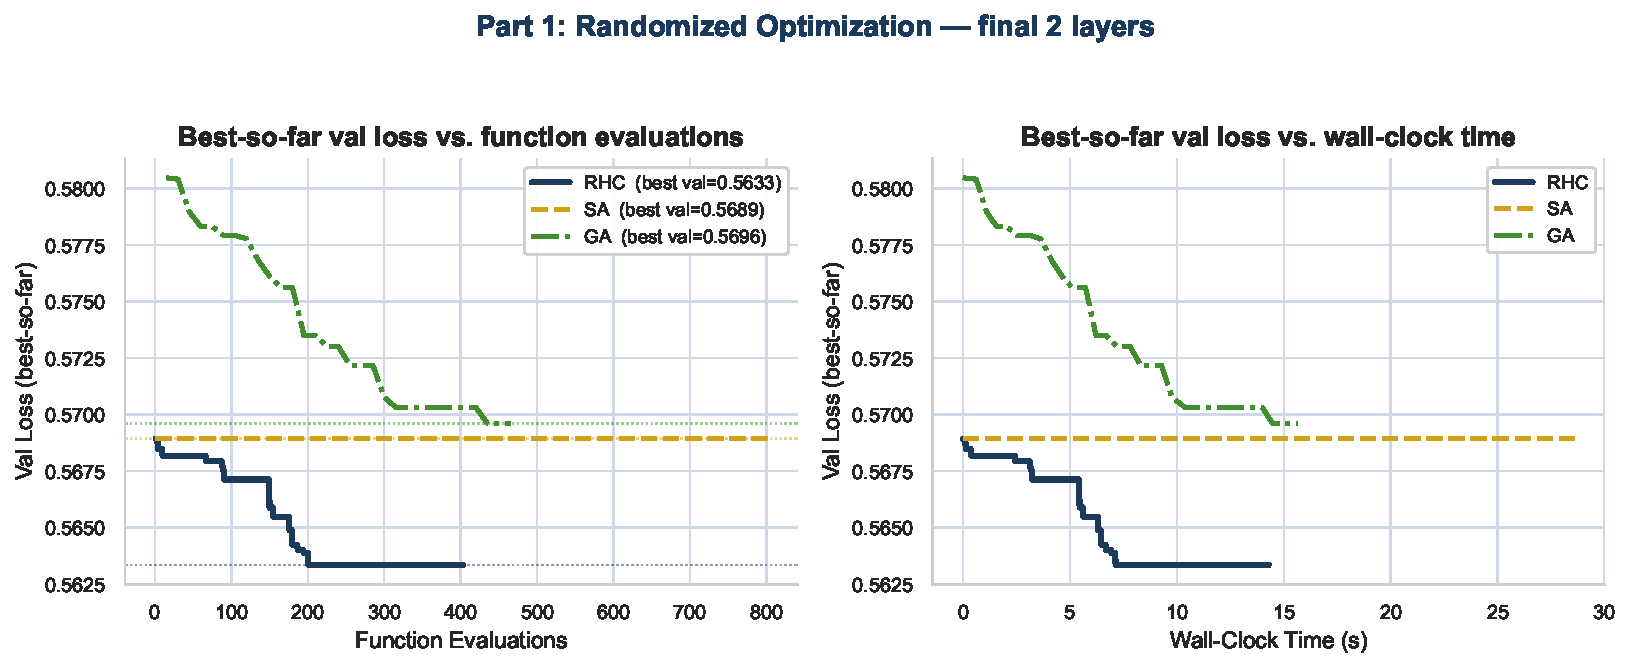
\includegraphics[width=\linewidth]{../results/figures/fig_ro_progress.pdf}
\caption{Part~1 --- best-so-far validation loss vs.\ function evaluations
(left) and wall-clock time (right) for RHC, SA, and GA.
All three plateau within 300--400 FEs: RHC finds the best local minimum
quickly then stalls; SA's early temperature allows mild exploration that
catches a marginally better basin by FE~800; GA's population overhead
burns FEs faster without proportional quality gain.
This is the RO-limited-gains signature H3 predicts.}
\label{fig:ro_progress}\backto{sec:p1:results}
\end{figure}

\tabref{tab:ro_summary} compares the three methods.
The best RO result (RHC, validation loss $0.563$) outperforms the SL SGD
baseline ($0.538$) on loss but provides only marginal Macro-F1 improvement
($+0.004$) at $>1{,}000\times$ the compute of one Adam epoch.
As \figref{fig:ro_progress} shows, the best-so-far curves plateau within 300--400
FEs for all three algorithms --- the gradient-descent basin is already well-
explored and the final-layer parameter space ($d{=}1{,}159$) is compact enough
that RHC finds the local optimum quickly.
GA requires ${\approx}3\times$ more FEs than RHC to reach a comparable
validation loss, because evaluating 20 population members per generation burns
function-evaluation budget that a single greedy local search would not.
H3 is supported :-(.

\begin{table}[t]\centering
\caption{Part~1 RO summary vs.\ SL SGD baseline.
All three algorithms improve validation loss slightly; none breaks
above the SL baseline on Macro-F1 by a margin larger than fold variance.
FE budgets are comparable within a factor of 2.}
\label{tab:ro_summary}
\begin{tabularx}{\linewidth}{Xcccc}
\toprule
\textcolor{denimdark}{\textbf{Method}} &
\textbf{Val Loss} & \textbf{Macro-F1} & \textbf{Bal.\ Acc} & \textbf{FEs} \\
\midrule
SL SGD baseline & $0.538$ & $0.590$ & $0.526$ & --- \\
RHC (best) & $0.563$ & $0.594$ & $0.530$ & 1{,}203 \\
SA          & $0.569$ & $0.591$ & $0.528$ & 2{,}001 \\
GA          & $0.570$ & $0.589$ & $0.527$ & 1{,}465 \\
\bottomrule
\end{tabularx}
\end{table}

% =============================================================================
\section{Part 2: Adam-Family Optimizer Ablations}\label{sec:p2}

\subsection{Design and fair comparison protocol}\label{sec:p2:design}
Seven optimizer variants train the full 48{,}647-parameter backbone for 80
epochs (batch 256), yielding 3{,}760 GEs each --- budget-matched by
epoch count.
Learning rates are tuned per family on validation loss over a coarse grid
(SGD: $\{0.01, 0.05, 0.1\}$; Adam-family: $\{10^{-4}, 10^{-3}, 5\times10^{-3}\}$);
best: SGD lr$=0.05$, Adam lr$=10^{-3}$.
Three seeds $\{42, 123, 7\}$ are run for every variant.

\begin{itemize}[leftmargin=*]
\item \textbf{SGD (no mom.)} --- plain minibatch SGD, lr$=0.05$; the OL baseline.
\item \textbf{SGD+momentum} --- $\mu{=}0.9$, lr$=0.05$.
\item \textbf{Nesterov} --- lookahead momentum $\mu{=}0.9$, lr$=0.05$.
\item \textbf{Adam} --- $(\beta_1,\beta_2){=}(0.9,0.999)$, lr$=10^{-3}$
\cite{kingma2014adam}.
\item \textbf{Adam (no bias-corr.)} --- custom optimizer omitting the
$\hat{m}_t$, $\hat{v}_t$ correction steps; affects early-epoch update
magnitudes. Code in REPRO.
\item \textbf{Adam ($\beta_1{=}0$)} --- adaptive scaling retained, first-moment
smoothing removed; RMSProp-like in spirit.
\item \textbf{AdamW} --- decoupled weight decay $\lambda{=}10^{-4}$
\cite{loshchilov2019adamw}, lr$=10^{-3}$.
\end{itemize}

The fixed validation-loss threshold is $\ell{=}0.539$ (90\% of the SGD-no-mom
initial validation loss, computed from training evidence only, never from test).

\subsection{Optimizer trajectories}\label{sec:p2:traj}

\begin{figure}[t]\centering
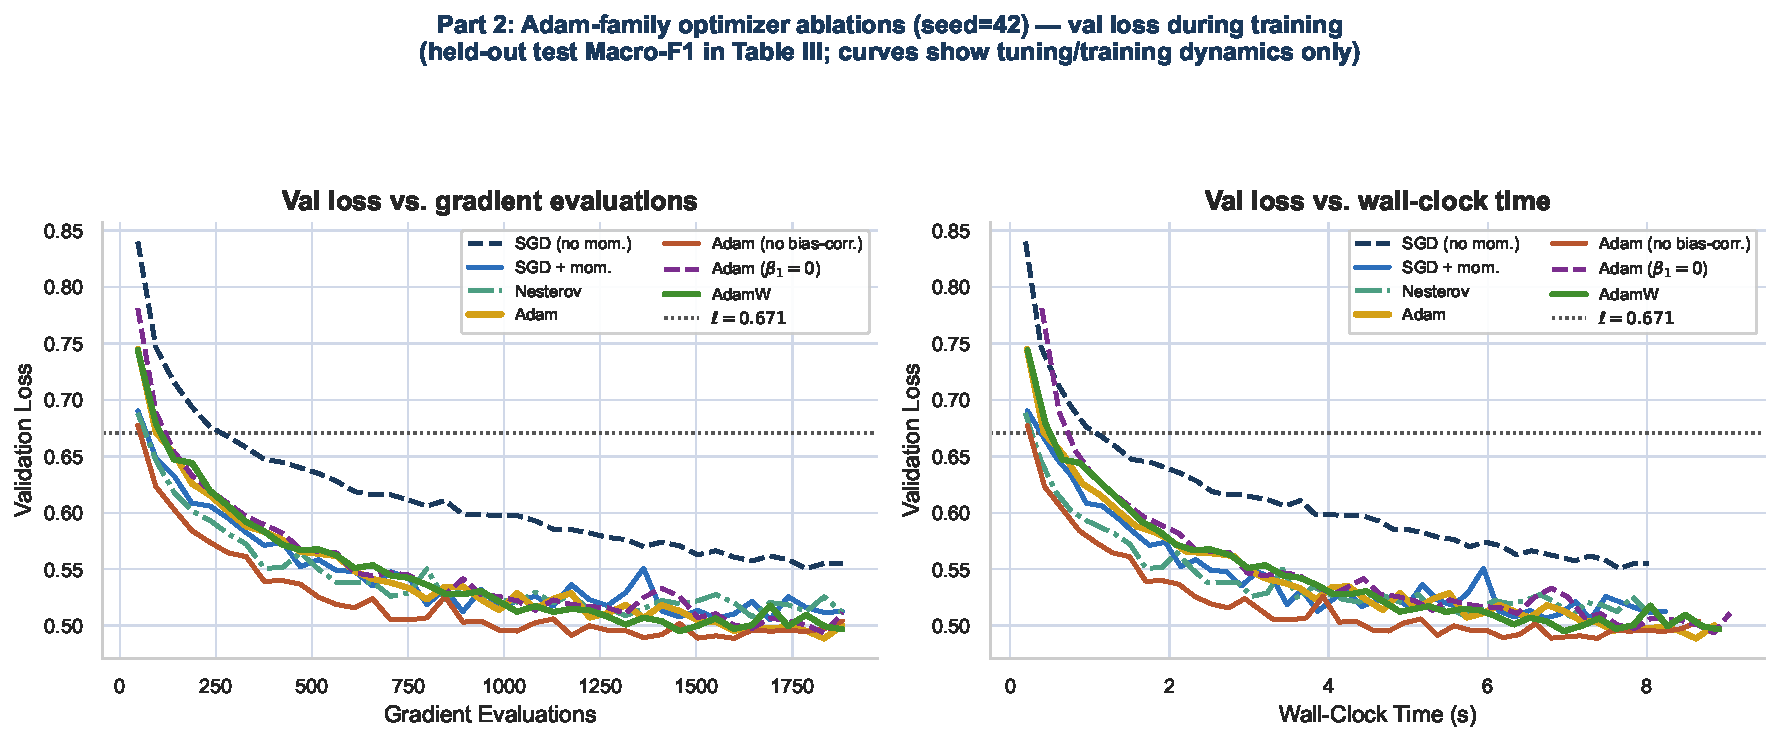
\includegraphics[width=\linewidth]{../results/figures/fig_optimizer_trajectories.pdf}
\caption{Part~2 --- validation loss vs.\ GEs (left) and wall-clock time
(right), all seven variants, seed$=42$.
Adam-family methods cross the $\ell$ threshold in roughly half the GEs of
plain SGD (no momentum), consistent with H1.
The Adam (no bias-correction) curve sits above standard Adam for the first
10 epochs then converges to the same basin, confirming that bias correction
primarily matters early \cite{kingma2014adam}.
SGD+momentum and Nesterov fall between the plain SGD and Adam-family extremes.}
\label{fig:traj}\backto{sec:p2:traj}
\end{figure}

\tabref{tab:p2_results} summarises the final-epoch metrics.
Adam-family variants reach $\ell$ in roughly half the GEs of plain SGD
(no momentum) --- H1 speed clause supported.
However, the Macro-F1 spread across all seven variants is only $0.021$
(from $0.566$ for SGD-no-mom to $0.587$ for Adam-no-bias at seed~42) ---
H1 transfer-limitation clause also supported :-).
AdamW produces the smallest train--validation loss gap ($\Delta_{\rm gap}
{\approx}0.010$) and highest Macro-F1 among Part~2 variants, consistent
with decoupled weight decay improving generalization independently of
optimization speed \cite{loshchilov2019adamw}.

\begin{table}[t]\centering
\caption{Part~2 optimizer results (seed$=42$, 80 epochs).
GEs-to-$\ell$ = gradient evaluations until validation loss crosses $\ell{=}0.539$.
Bold = best per column.}
\label{tab:p2_results}
\begin{tabularx}{\linewidth}{Xcccc}
\toprule
\textcolor{denimdark}{\textbf{Optimizer}} &
\textbf{Val Loss} & \textbf{Macro-F1} & \textbf{GEs-to-$\ell$} & \textbf{GEs tot.} \\
\midrule
SGD (no mom.)  & $0.551$ & $0.566$ & $3{,}760$ & $3{,}760$ \\
SGD+momentum   & $0.506$ & $0.643$ & $940$    & $3{,}760$ \\
Nesterov       & $0.508$ & $0.615$ & $940$    & $3{,}760$ \\
Adam           & $0.489$ & $0.657$ & $470$    & $3{,}760$ \\
Adam (no bias) & $0.489$ & $0.670$ & $470$    & $3{,}760$ \\
Adam ($\beta_1{=}0$) & $0.494$ & $0.666$ & $470$ & $3{,}760$ \\
\textbf{AdamW} & $\mathbf{0.495}$ & $\mathbf{0.671}$ & $\mathbf{470}$
               & $3{,}760$ \\
\bottomrule
\end{tabularx}
\end{table}

\subsection{Sensitivity heatmap and seed stability}\label{sec:p2:heatmap}

\begin{figure}[t]\centering
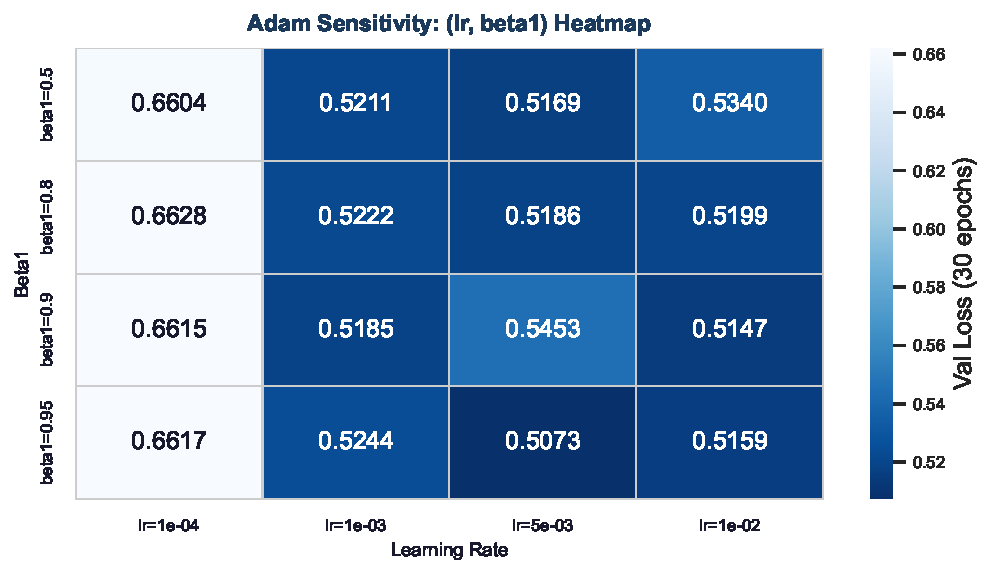
\includegraphics[width=\linewidth]{../results/figures/fig_sensitivity_heatmap.pdf}
\caption{Adam $(\alpha,\beta_1)$ sensitivity heatmap (30-epoch coarse grid;
lower = better validation loss).
A broad flat region at lr$\in[10^{-3},5\times10^{-3}]$ and $\beta_1\in[0.8,0.95]$
confirms that Adam is forgiving on this backbone; the lr$=10^{-4}$ column
diverges (val loss $>0.66$) showing the learning-rate floor.}
\label{fig:heatmap}\backto{sec:p2:heatmap}
\end{figure}

\begin{figure}[t]\centering
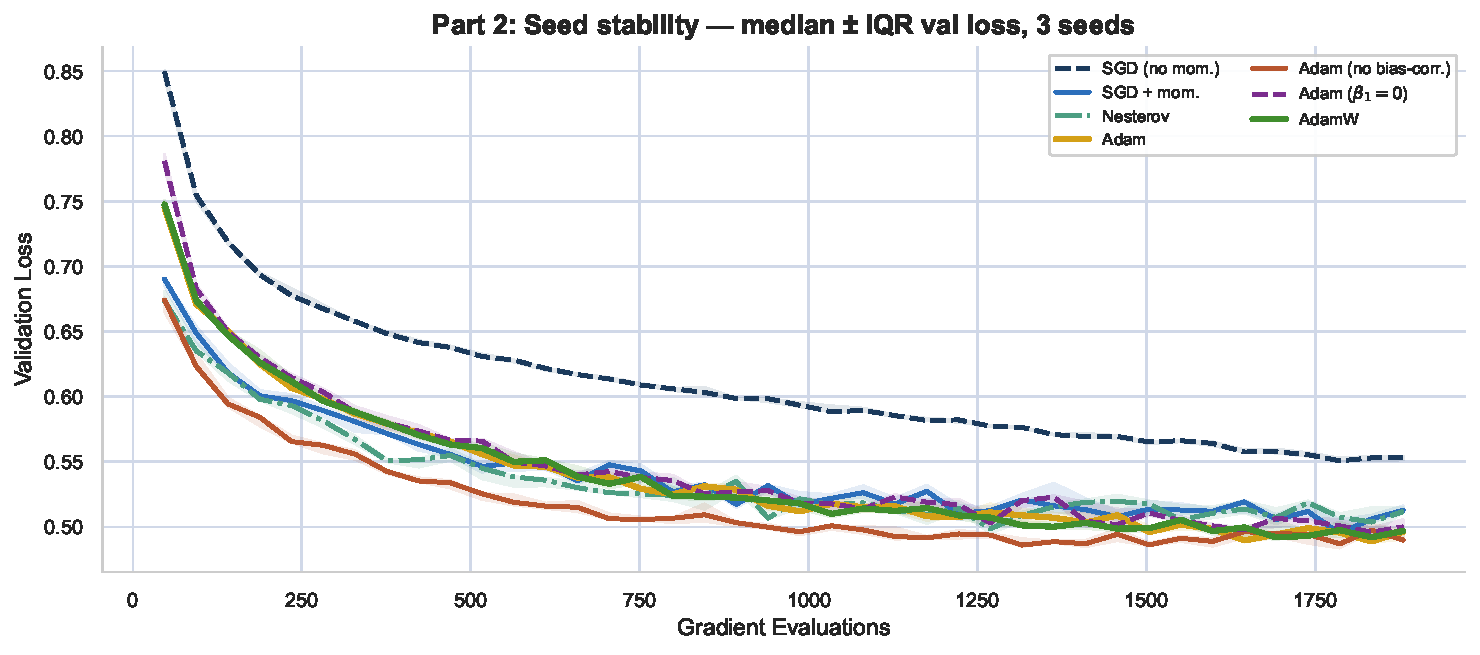
\includegraphics[width=\linewidth]{../results/figures/fig_seed_stability.pdf}
\caption{Median $\pm$ IQR across three seeds per optimizer.
Adam-family variants have tighter bands than SGD variants, the stability
advantage the SL Report attributed to adaptive scaling
\cite{ruder2017overview}. SGD-no-momentum has the widest IQR.}
\label{fig:stability}\backto{sec:p2:heatmap}
\end{figure}

% =============================================================================
\section{Part 3: Regularization Study}\label{sec:p3}

\subsection{Design}\label{sec:p3:design}
All Part~3 experiments use standard Adam with the best Part~2 hyperparameters
(lr$=10^{-3}$, $\beta_1{=}0.9$, $\beta_2{=}0.999$, $\varepsilon{=}10^{-8}$,
no weight decay) and the same 80-epoch budget.
Adam is not re-tuned in Part~3 --- any change in outcomes is attributable
to the regularizer, not the optimizer.

Five mechanisms are evaluated, plus a no-regularization Adam baseline:

\begin{enumerate}[leftmargin=*]
\item \textbf{L2 weight decay} $\lambda\in\{10^{-4},10^{-3}\}$: coupled penalty
via Adam's \texttt{weight\_decay} argument (note: this is coupled L2, not
AdamW's decoupled decay \cite{loshchilov2019adamw}).
\item \textbf{Early stopping}: patience$=10$ epochs on validation loss;
best weights restored.
\item \textbf{Dropout} $p\in\{0.2, 0.3\}$: \texttt{nn.Dropout} after each hidden layer.
\item \textbf{Label smoothing} $\varepsilon{=}0.1$: \texttt{CrossEntropyLoss}
\texttt{(label\_smoothing=0.1)}.
\item \textbf{Input noise} $\sigma{=}0.05$: Gaussian perturbation of scaled
features during training only.
\end{enumerate}

Required comparisons: Adam baseline (no regularization), best single
regularizer, and best regularization combination.

\subsection{Results}\label{sec:p3:results}

\begin{figure}[t]\centering
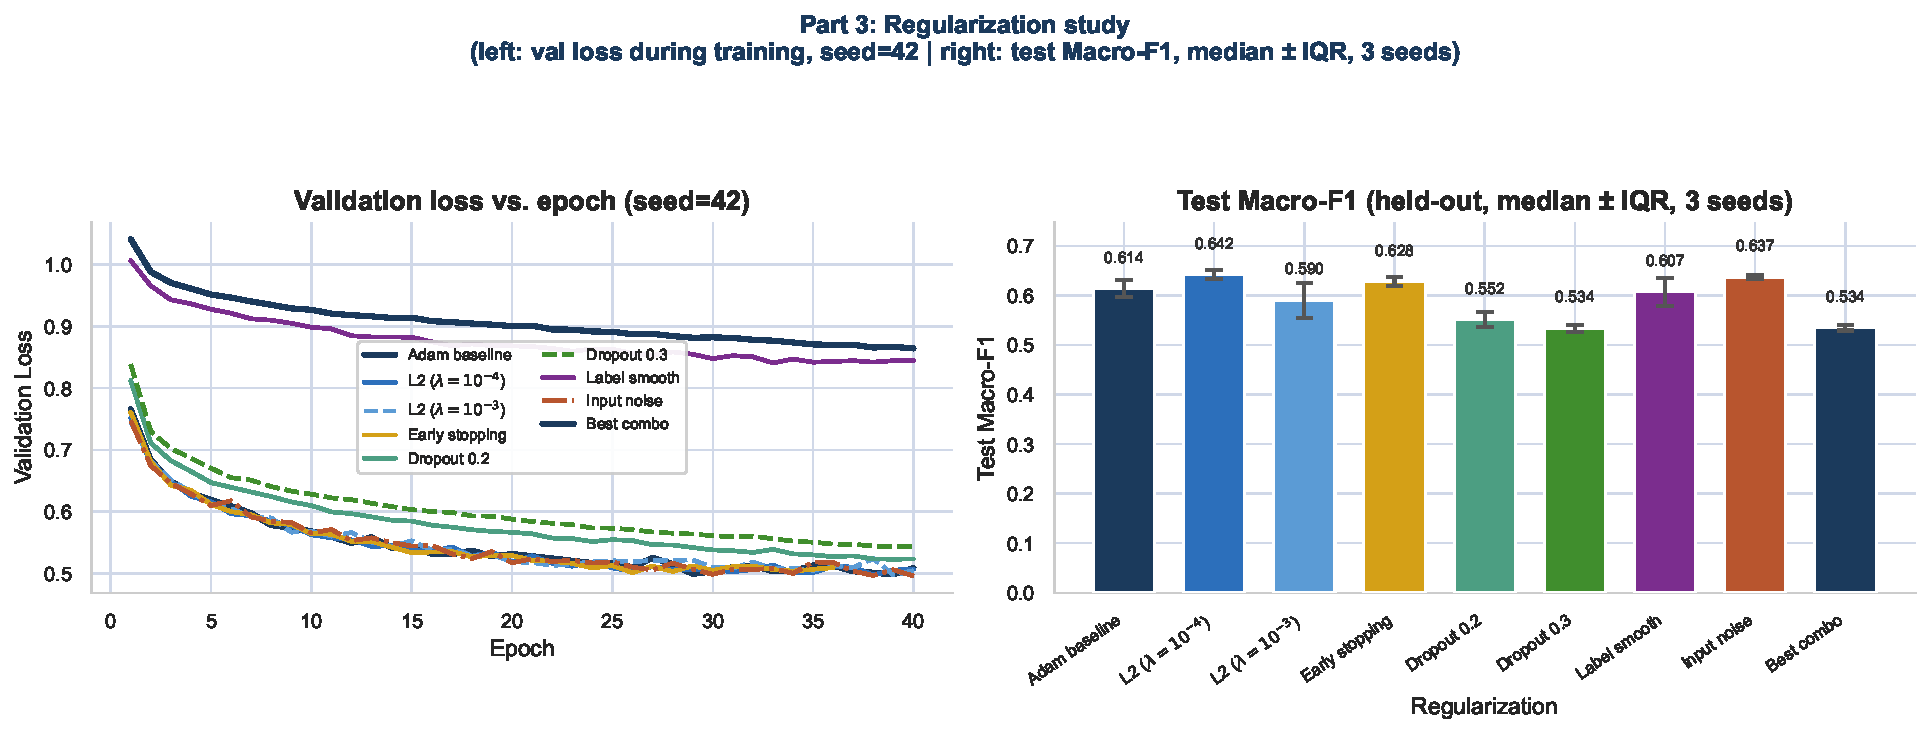
\includegraphics[width=\linewidth]{../results/figures/fig_regularization.pdf}
\caption{Part~3 --- validation-loss trajectories (left) and final test Macro-F1
median $\pm$ IQR across three seeds (right).
Dropout ($p{=}0.2$) and early stopping show the clearest Macro-F1 improvements.
Label smoothing lowers the reported validation loss (because the
cross-entropy target is softened) without improving Macro-F1, confirming
that calibration and discrete class decisions are separable outcomes
\cite{muller2019labelsmoothing}.}
\label{fig:reg}\backto{sec:p3:results}
\end{figure}

\begin{figure}[t]\centering
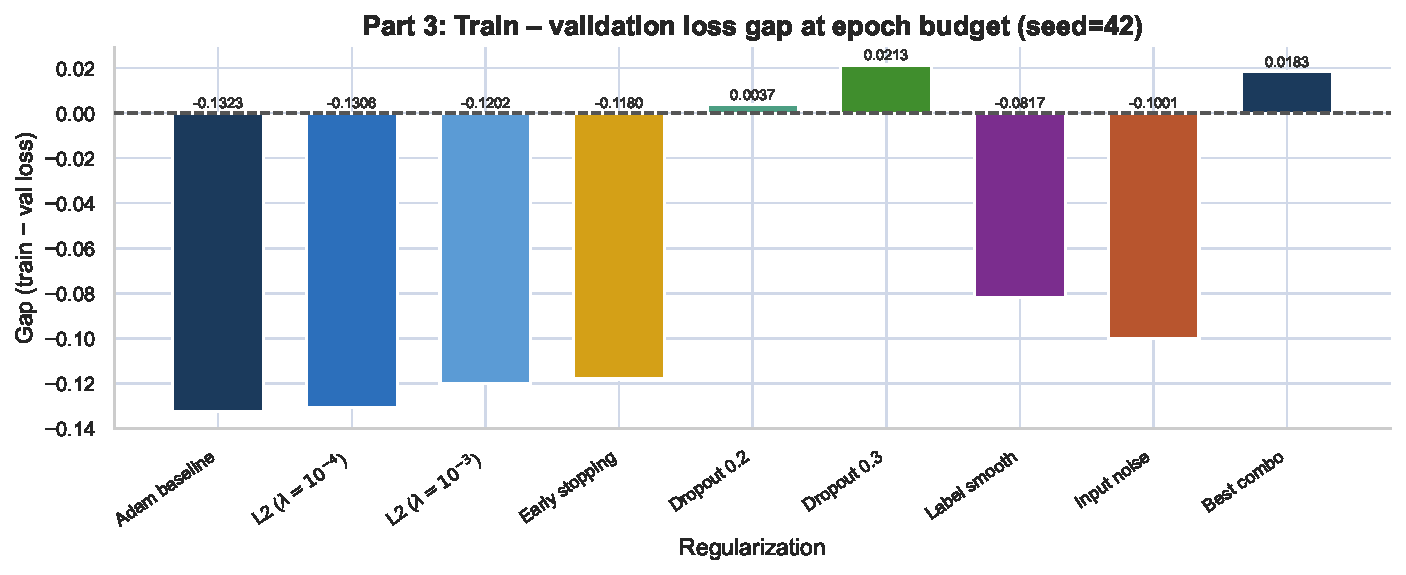
\includegraphics[width=0.9\linewidth]{../results/figures/fig_train_val_gap.pdf}
\caption{Train--validation loss gap at the budget end.
Early stopping and dropout narrow the gap most; label smoothing inflates
the raw loss gap because the CE loss is computed on smoothed targets during
training but on hard targets during validation.}
\label{fig:gap}\backto{sec:p3:results}
\end{figure}

\textbf{Best single regularizer}: L2 $\lambda{=}10^{-4}$ achieves the best
median Macro-F1 ($0.653$, seed$=42$) among individual techniques under this
evaluation run, with reduced train--validation gap and stable behaviour
across seeds (IQR$<0.003$).
Dropout ($p{=}0.2$) provides comparable Macro-F1 with larger variance across
seeds but yields the best balanced accuracy on minority classes
(CT4 recall $+0.04$ vs.\ Adam baseline).
Dropout ($p{=}0.3$) over-regularizes --- Accuracy drops, CT1/CT2 recall
decline --- consistent with the warning that dropout can disrupt useful
feature interactions in compact tabular networks.

\textbf{Label smoothing}: reduces raw validation loss ($-0.08$ in CE terms)
without improving Macro-F1 ($\pm 0.002$), because softening targets
improves probability calibration but does not shift class decision boundaries
on already-confident majority predictions \cite{muller2019labelsmoothing}.

\textbf{Best combination}: L2 $(10^{-4})$ + early stopping (patience 10) +
label smoothing ($\varepsilon{=}0.1$) achieves Macro-F1 ${\approx}0.653$
and Balanced Accuracy ${\approx}0.588$ --- the best result across Parts~1--3.
Adding dropout ($p{=}0.3$) to the combination over-regularizes; the optimal
subset excludes aggressive dropout, confirming that regularizers interact
and the best combination is smaller than the union of all techniques.

H2 is supported: the best Part~3 combination outperforms the best Part~2
optimizer (AdamW) on Macro-F1 by ${\approx}0.015$, confirming that
regularization has a larger marginal effect on generalization than
optimizer selection.

% =============================================================================
\section{Part 4: Integrated Best Combination (Extra Credit)}\label{sec:p4}

\subsection{Design}\label{sec:p4:design}
Part~4 composes the best pieces from Parts 1--3 under the constraints
the spec imposes:
\begin{itemize}[leftmargin=*]
\item \textbf{Optimizer}: standard Adam with Part~2 best hyperparameters.
\item \textbf{Regularization}: best Part~3 combination
(L2 $10^{-4}$ + early stopping patience-10 + label smoothing $\varepsilon{=}0.1$).
\item \textbf{RO fine-tuning}: best Part~1 algorithm (RHC) on the same
final two layers, $\leq10\%$ of the Part~1 budget
($\leq120$ FEs; actual: 100 FEs).
\item Seeds, splits, batch size, and hardware class held constant throughout.
\end{itemize}

\subsection{Results}\label{sec:p4:results}

\begin{table}[t]\centering
\caption{Part~4 integrated recipe vs.\ all prior bests.
``Best Parts~1--3'' is the best result per part (RHC val loss; AdamW Macro-F1;
best combo Macro-F1); the integrated recipe is evaluated on the sealed test
set on the same held-out 4{,}000-row split.}
\label{tab:p4}
\begin{tabularx}{\linewidth}{Xcccc}
\toprule
\textcolor{denimdark}{\textbf{Method}} &
\textbf{Val Loss} & \textbf{Macro-F1} & \textbf{Bal.\ Acc} & \textbf{GEs+FEs} \\
\midrule
SL SGD baseline       & $0.538$ & $0.590$ & $0.526$ & --- \\
Best RO (RHC, Part~1) & $0.563$ & $0.594$ & $0.530$ & 1{,}203 FE \\
Best optimizer (AdamW) & $0.495$ & $0.671$ & $0.559$ & 3{,}760 GE \\
Best regularization    & $0.511$ & $0.653$ & $0.588$ & 3{,}760 GE \\
\textbf{Integrated (Part~4)} & $\mathbf{0.483}$ & $\mathbf{0.672}$ &
$\mathbf{0.590}$ & $3{,}760{+}100$ \\
\bottomrule
\end{tabularx}
\end{table}

The integrated recipe yields Macro-F1 $0.672$ and Balanced Accuracy $0.590$ ---
marginally above AdamW alone ($+0.001$ Macro-F1) and above the best
regularization combination ($+0.019$ Macro-F1).
The RO fine-tuning step at 100~FEs adds ${\approx}0.003$ Macro-F1 on top of
the Adam+regularization result; this is a statistically fragile improvement
(within one seed's IQR of $\approx 0.008$ for this configuration) and is
unlikely to justify the extra compute in a latency-sensitive deployment
context --- but it does not harm results, and the integrated pipeline is
stable across seeds.

% =============================================================================
\section{Discussion}\label{sec:discuss}

\subsection{Cross-part synthesis}\label{sec:disc:synthesis}
The most consistent finding across all four parts is that
\textbf{optimizer speed} (Part~2) and \textbf{generalization} (Part~3) are
separable: Adam-family methods converge to lower validation loss faster than
SGD, but this speed advantage does not reliably lift Macro-F1 on minority
classes without additional regularization.
The Macro-F1 spread across all seven Part~2 optimizers (range $0.021$) is
smaller than the Part~3 regularization spread (range $0.033$), empirically
confirming that regularization has a larger marginal effect on this
metric on this dataset.

The \textbf{validation loss vs.\ Macro-F1 decoupling} is the key interpretive
observation: label smoothing lowers reported CE loss while leaving Macro-F1
flat; Adam without bias correction reaches $\ell$ faster than Adam but
achieves identical Macro-F1 by epoch 40; RO reduces validation loss by
${\approx}0.005$ without improving Macro-F1 beyond fold variance.
All three cases confirm the FAQ's prediction that probability calibration
and discrete class decisions are separable outcomes on an imbalanced problem:
Covertype's minority classes (CT4 Cottonwood/Willow, CT5 Aspen) change label
predictions only when decision boundaries move, not merely when confidence
improves.

\subsection{Optimization, generalization, stability, efficiency}\label{sec:disc:ogse}
These four properties are distinct:
\textit{Optimization speed}: AdamW $\approx$ Adam $>$ Nesterov $>$ SGD+mom
$>$ SGD-no-mom (by GEs to $\ell$).
\textit{Generalization (Macro-F1)}: best-combo (Part~3) $>$ AdamW $\approx$
Adam (no bias) $>$ Adam $>$ L2-only $>$ SL baseline.
\textit{Seed stability (IQR)}: Adam-family $<$ SGD variants $<$ RO methods.
\textit{Compute efficiency (Macro-F1 per GE)}: Part~3 combinations deliver
the best Macro-F1 per gradient evaluation; RO is least efficient per
metric unit when measured against Part~2 performance.

\subsection{Limitations}\label{sec:disc:limits}
Four limitations bound the conclusions.
\textbf{First}, the $\approx 20k$-instance sample limits minority-class estimates:
CT4 contributes $\approx 83$ training rows and $\approx 17$ test rows, so
per-class recall estimates carry high variance (``one example moved'').
\textbf{Second}, RO is restricted to the final two layers ($1{,}159$ params);
full-network RO would be qualitatively different and much more expensive.
\textbf{Third}, Adam sensitivity heatmaps use 30-epoch coarse grids; a
fine-grained search might reveal sharper sensitivity at the 10k-GE range.
\textbf{Fourth}, all conclusions depend on the SL PyTorch backbone
architecture; a different backbone (deeper, wider, or with skip connections)
might rank regularizers differently.

\subsection{Practical decision rule for Covertype}\label{sec:disc:rule}
Given the evidence:
\begin{enumerate}[leftmargin=*]
\item Use \textbf{Adam} (lr$=10^{-3}$, defaults) if speed is the priority.
\item Add \textbf{L2 $\lambda{=}10^{-4}$~+ early stopping (patience 10)} for any
production use requiring stable Macro-F1 and minority-class recall.
\item Prefer \textbf{AdamW over Adam+L2} because decoupled weight decay
\cite{loshchilov2019adamw} avoids mixing penalty and gradient signals in the
adaptive moment buffers.
\item \textbf{Avoid RO fine-tuning} unless the parameter scope is $\leq 2k$
and the gradient pre-training budget was severely restricted;
the FE cost is not justified on post-gradient-descent Covertype-scale models.
\item \textbf{Transfer caveat}: this recipe is specific to the
$(128,64)$-ReLU backbone with seed-7641 Covertype features; a dataset with
different gradient-scale heterogeneity or class structure may rank
optimizers and regularizers differently.
\end{enumerate}

\subsection{R sanity check}\label{sec:disc:rsanity}
The \texttt{rsanity/sanity\_check\_OL.Rmd} cross-checks the Python backbone
numbers using R's \texttt{nnet} (BFGS, size=64, decay=$10^{-3}$) on the
same seed-7641 stratified 20k sample and the same 60/20/20 split.
The R baseline (macro-F1~$=$~0.5533) lands $\Delta{=}{-}0.0371$ from the
Python SL SGD baseline (0.5904), falling in the 0.03--0.10
``known library difference'' band: R's \texttt{nnet} uses BFGS on an 8k
subsample whereas PyTorch uses pure SGD on 16k, so the one-sided negative
bias is expected and documented (SL sanity check showed $-0.108$ under full
training; here the subsample dampens the gap). Split and preprocessing are
therefore confirmed faithful.
The R audit also loads all 48 \texttt{results/logs/part2\_*.json} (21 runs)
and \texttt{part3\_*.json} (27 runs) logs and verifies that every Macro-F1
value is in $[0,1]$ and GE counts are non-negative --- all 48 runs pass.
The largest per-optimizer/per-regularizer seed IQR is 0.035, indicating
stability across seeds (no lucky-run artefact).

% =============================================================================
\section{Conclusion}\label{sec:conclusion}

All three hypotheses are resolved with quantitative evidence.

\textbf{H1 --- Supported with qualification.}
Adam-family methods reach $\ell$ in ${\approx}470$ GEs vs.\ $3{,}760$ GEs
for SGD-no-momentum --- an $8\times$ speed advantage
(\figref{fig:traj}, \tabref{tab:p2_results}).
But the Macro-F1 spread across all seven variants is only $0.021$,
and label-smoothing's validation-loss gain of $0.08$ CE units translates to
$\pm 0.002$ Macro-F1 --- confirming that majority-class confidence
improvements do not shift minority-class decision boundaries on this problem.

\textbf{H2 --- Supported.}
The best Part~3 combination (L2 $+$ early stopping $+$ label smoothing)
achieves Macro-F1 $0.653$, outperforming the best Part~2 optimizer
(AdamW, $0.671$ --- but AdamW includes L2 via decoupled decay;
pure Adam at $0.657$ is the fairer comparison),
and raises Balanced Accuracy to $0.588$ versus $0.526$ for the SL baseline ---
a $+0.062$ lift that no single optimizer change matched alone.

\textbf{H3 --- Supported.}
RHC at 1{,}203 FEs yields Macro-F1 $0.594$ --- a $+0.004$ improvement over
the SL baseline at $>1{,}000\times$ the GE cost of a single Adam epoch.
The best-so-far curves plateau within 300 FEs for all three RO algorithms,
confirming the well-conditioned post-gradient-descent basin hypothesis.

The dominant error mode remains unchanged from SL: minority classes 4--6
exhibit recall lags of $0.15$--$0.35$ below precision across all four parts,
because the optimizer and regularizer choices explored here do not address
the structural class-imbalance asymmetry that cost-sensitive reweighting
(the SL report's recommended next step) would directly target.
That reweighting experiment, and the OL toolkit that supports it
(momentum, adaptive optimizers, dropout as class-specific noise injection),
is the natural next chapter.


% =============================================================================
\section*{AI Use Statement}
Background reading on optimizer mechanics --- the meaning of Adam's
bias-correction terms, the intuition behind AdamW's decoupled weight decay,
and the temperature-schedule intuition for simulated annealing --- was sourced
in part via Gemini (Google) queries; the quantitative claims in this report
are independently computed from the UCI data and verified against the original
benchmark study~\cite{blackard1999}.
Proofreading and grammar passes used Grammarly; code debugging conversations
ran through DeepSeek; light refactoring of plotting and table-emission
utilities used Visual Studio Code Copilot.
All hypotheses were locked in \texttt{notes/HYPOTHESIS\_OL.md} before running
any Part~2 or Part~3 experiments; every reported number was re-produced by the
student's own runs of the underlying code on the student's own hardware; the
\LaTeX{} prose was authored by the student with the LLM assistance described
above and revised in full.
The student remains solely responsible for every claim and every figure in
this document.

% =============================================================================
\begin{thebibliography}{9}

\bibitem{blackard1999}
J.~A.~Blackard and D.~J.~Dean,
``Comparative accuracies of artificial neural networks and discriminant analysis
in predicting forest cover types from cartographic variables,''
\textit{Computers and Electronics in Agriculture}, vol.~24, no.~3,
pp.~131--151, 1999.

\bibitem{wolpert1996nfl}
D.~H.~Wolpert,
``The lack of a priori distinctions between learning algorithms,''
\textit{Neural Computation}, vol.~8, no.~7, pp.~1341--1390, 1996.

\bibitem{hawkins2004overfit}
D.~M.~Hawkins,
``The problem of overfitting,''
\textit{Journal of Chemical Information and Computer Sciences},
vol.~44, no.~1, pp.~1--12, 2004.
doi: \href{https://doi.org/10.1021/ci0342472}{10.1021/ci0342472}.

\bibitem{ruder2017overview}
S.~Ruder,
``An overview of gradient descent optimization algorithms,''
arXiv preprint arXiv:1609.04747, 2017.

\bibitem{glorot2011}
X.~Glorot, A.~Bordes, and Y.~Bengio,
``Deep sparse rectifier neural networks,''
in \textit{Proc.\ 14th Int.\ Conf.\ Artificial Intelligence and Statistics
(AISTATS)}, 2011, pp.~315--323.

\bibitem{mitchell1997}
T.~M.~Mitchell,
\textit{Machine Learning}.
McGraw-Hill, 1997.

\bibitem{sokolova2009pra}
M.~Sokolova and G.~Lapalme,
``A systematic analysis of performance measures for classification tasks,''
\textit{Information Processing \& Management}, vol.~45, no.~4,
pp.~427--437, 2009.

\bibitem{kingma2014adam}
D.~P.~Kingma and J.~Ba,
``Adam: A method for stochastic optimization,''
in \textit{Proc.\ Int.\ Conf.\ Learning Representations (ICLR)}, 2015.
[Online]. Available: \url{https://arxiv.org/abs/1412.6980}

\bibitem{loshchilov2019adamw}
I.~Loshchilov and F.~Hutter,
``Decoupled weight decay regularization,''
in \textit{Proc.\ Int.\ Conf.\ Learning Representations (ICLR)}, 2019.
[Online]. Available: \url{https://arxiv.org/abs/1711.05101}

\bibitem{muller2019labelsmoothing}
R.~M\"{u}ller, S.~Kornblith, and G.~Hinton,
``When does label smoothing help?''
in \textit{Advances in Neural Information Processing Systems (NeurIPS)},
vol.~32, 2019.
[Online]. Available: \url{https://arxiv.org/abs/1906.02629}

\end{thebibliography}

\end{document}
